\documentclass{beamer}
\usetheme{metropolis}
\usepackage{graphicx}
\usepackage{amsmath}
\usepackage{makecell}
\title{A History of Science in Latin America (INTD290): Unit 1.2}
\author{Jordan Hanson}
\institute{Whittier College Department of Physics and Astronomy}

\begin{document}
\maketitle

\section{Outline}

\begin{frame}{Outline}
\textit{Comparitive medical treatments - chapter 1 content.} \\
\alert{Chapter 2 content}
\begin{enumerate}
\item Mining and agriculture in Nueva Espa\~{n}a
\item Construction of scientific communities
\item The formation of scientific literature and community, importation of scientific texts
\item Catholic religious orders in Latin America
\item Galileo, Kepler, and the Heliocentric system of the world
\end{enumerate}
\alert{Activities}
\begin{enumerate}
\item Timelines of discoveries and development
\item Geographical illustrations with Google Earth
\item Digital Storytelling on cosmic rays and the solar wind
\end{enumerate}
\end{frame}

\section{More on Literary Societies and Journals}

\begin{frame}{More on Literary Societies and Journals}
\small
\begin{figure}
\centering
\includegraphics[width=0.95\textwidth]{figures/TimeLine1.pdf}
\caption{\label{fig:time1} A visualization of scientific journals of the 18th Century Latin American society.  Note the prevalance of Societies of Friends of the Country, versus Royal Societies.  Note also the gap between 1700-1750.  For a complete list of journals in the gap, see the link at lower left.}
\end{figure}
\end{frame}

\begin{frame}{More on Literary Societies and Journals}
\small
\begin{enumerate}
\item Friends of the Country versus Royal Society
\item Alzate, Bartolache (Mexico)
\item Other journals not shown: \textit{Gacetas de Caracas, 1808}, \textit{Semenario de Agricultura, Industria y Comercio, Buenos Aires, 1802}, \textit{O Patriota, 1813-1814}
\item Mining processes debated in these journals, the patio process versus the Born process
\begin{itemize}
\item Fausto de Elh\'{u}yar (Spain), Baron von Nordenflicht (Sweden)
\item Jos\'{e} Antonio Alzate (New Spain) wrote in \textit{Observaciones} in 1787 that \'{A}lvaro Alonso Barba discovered the ``Born method'' in 1640.  The Creoles noted that the Born method was not as efficient in this situation.
\end{itemize}
\end{enumerate}
\end{frame}

\begin{frame}{More on Literary Societies and Journals}
The results of an intriguing physics experiment were first published in \textbf{Gacetas de Literatura}, by Jos\'{e} Antonio Alzate y Ram\'{i}rez, Jos\'{e} Francisco Dimas Rangel, and Antonio de Le\'{o}n y Gama.  An article summarizing their results: \\ \vspace{0.5cm}
M. P. Ramos-Lara \textit{Contribuciones de astrónomos mexicanos al estudio de auroras boreales de baja latitud entre 1789 y 1791}.  Revista Mexicana de F\'{i}sica E \textbf{18} (1) 156-167 \\ \vspace{0.5cm}
\url{https://youtu.be/czMh3BnHFHQ} \\
\url{https://xkcd.com/2004/}
\end{frame}

\begin{frame}[fragile]{More on Literary Societies and Journals}
\small
\begin{columns}
\begin{column}{0.5\textwidth}
\textbf{\alert{Jos\'{e} Antonio Alzate y Ram\'{i}rez}}
\begin{enumerate}
\item Catholic priest, and descended from Juana In\'{e}z de La Cruz (protofeminist Catholic nun, writer, intellectual - see the work of Octavio Paz).
\item Meteorology, Physics, Astronomy, Mathematics, Indigenous history
\item Corresponding member of French and Spanish Academies of Science
\end{enumerate}
\end{column}
\begin{column}{0.5\textwidth}
\begin{figure}
\centering
\includegraphics[width=2cm]{figures/Jose_antonio_alzate_ramirez.jpg}
\end{figure}
\begin{itemize}
\item Wrote 30 books.  One of them: \textit{Observaci\'{o}n del paso de Venus por el disco del Sol.} (1770)
\item 1885: La Sociedad Científica Antonio Alzate, later became The National Academy of Sciences (Mexico)
\end{itemize}
\end{column}
\end{columns}
\end{frame}

\begin{frame}[fragile]{More on Literary Societies and Journals}
\small
\begin{columns}
\begin{column}{0.5\textwidth}
\textbf{\alert{Antonio de Le\'{o}n y Gama}}
\begin{enumerate}
\item Lawyer who worked at the \textit{Real Audiencia de M\'{e}xico}
\item Astronomer, anthropologist, writer, watchmaker
\item Discovered two important anthropological items:
\item (Projects?)
\end{enumerate}
\end{column}
\begin{column}{0.5\textwidth}
\begin{figure}
\centering
\includegraphics[width=2cm]{figures/leonygama.jpeg}
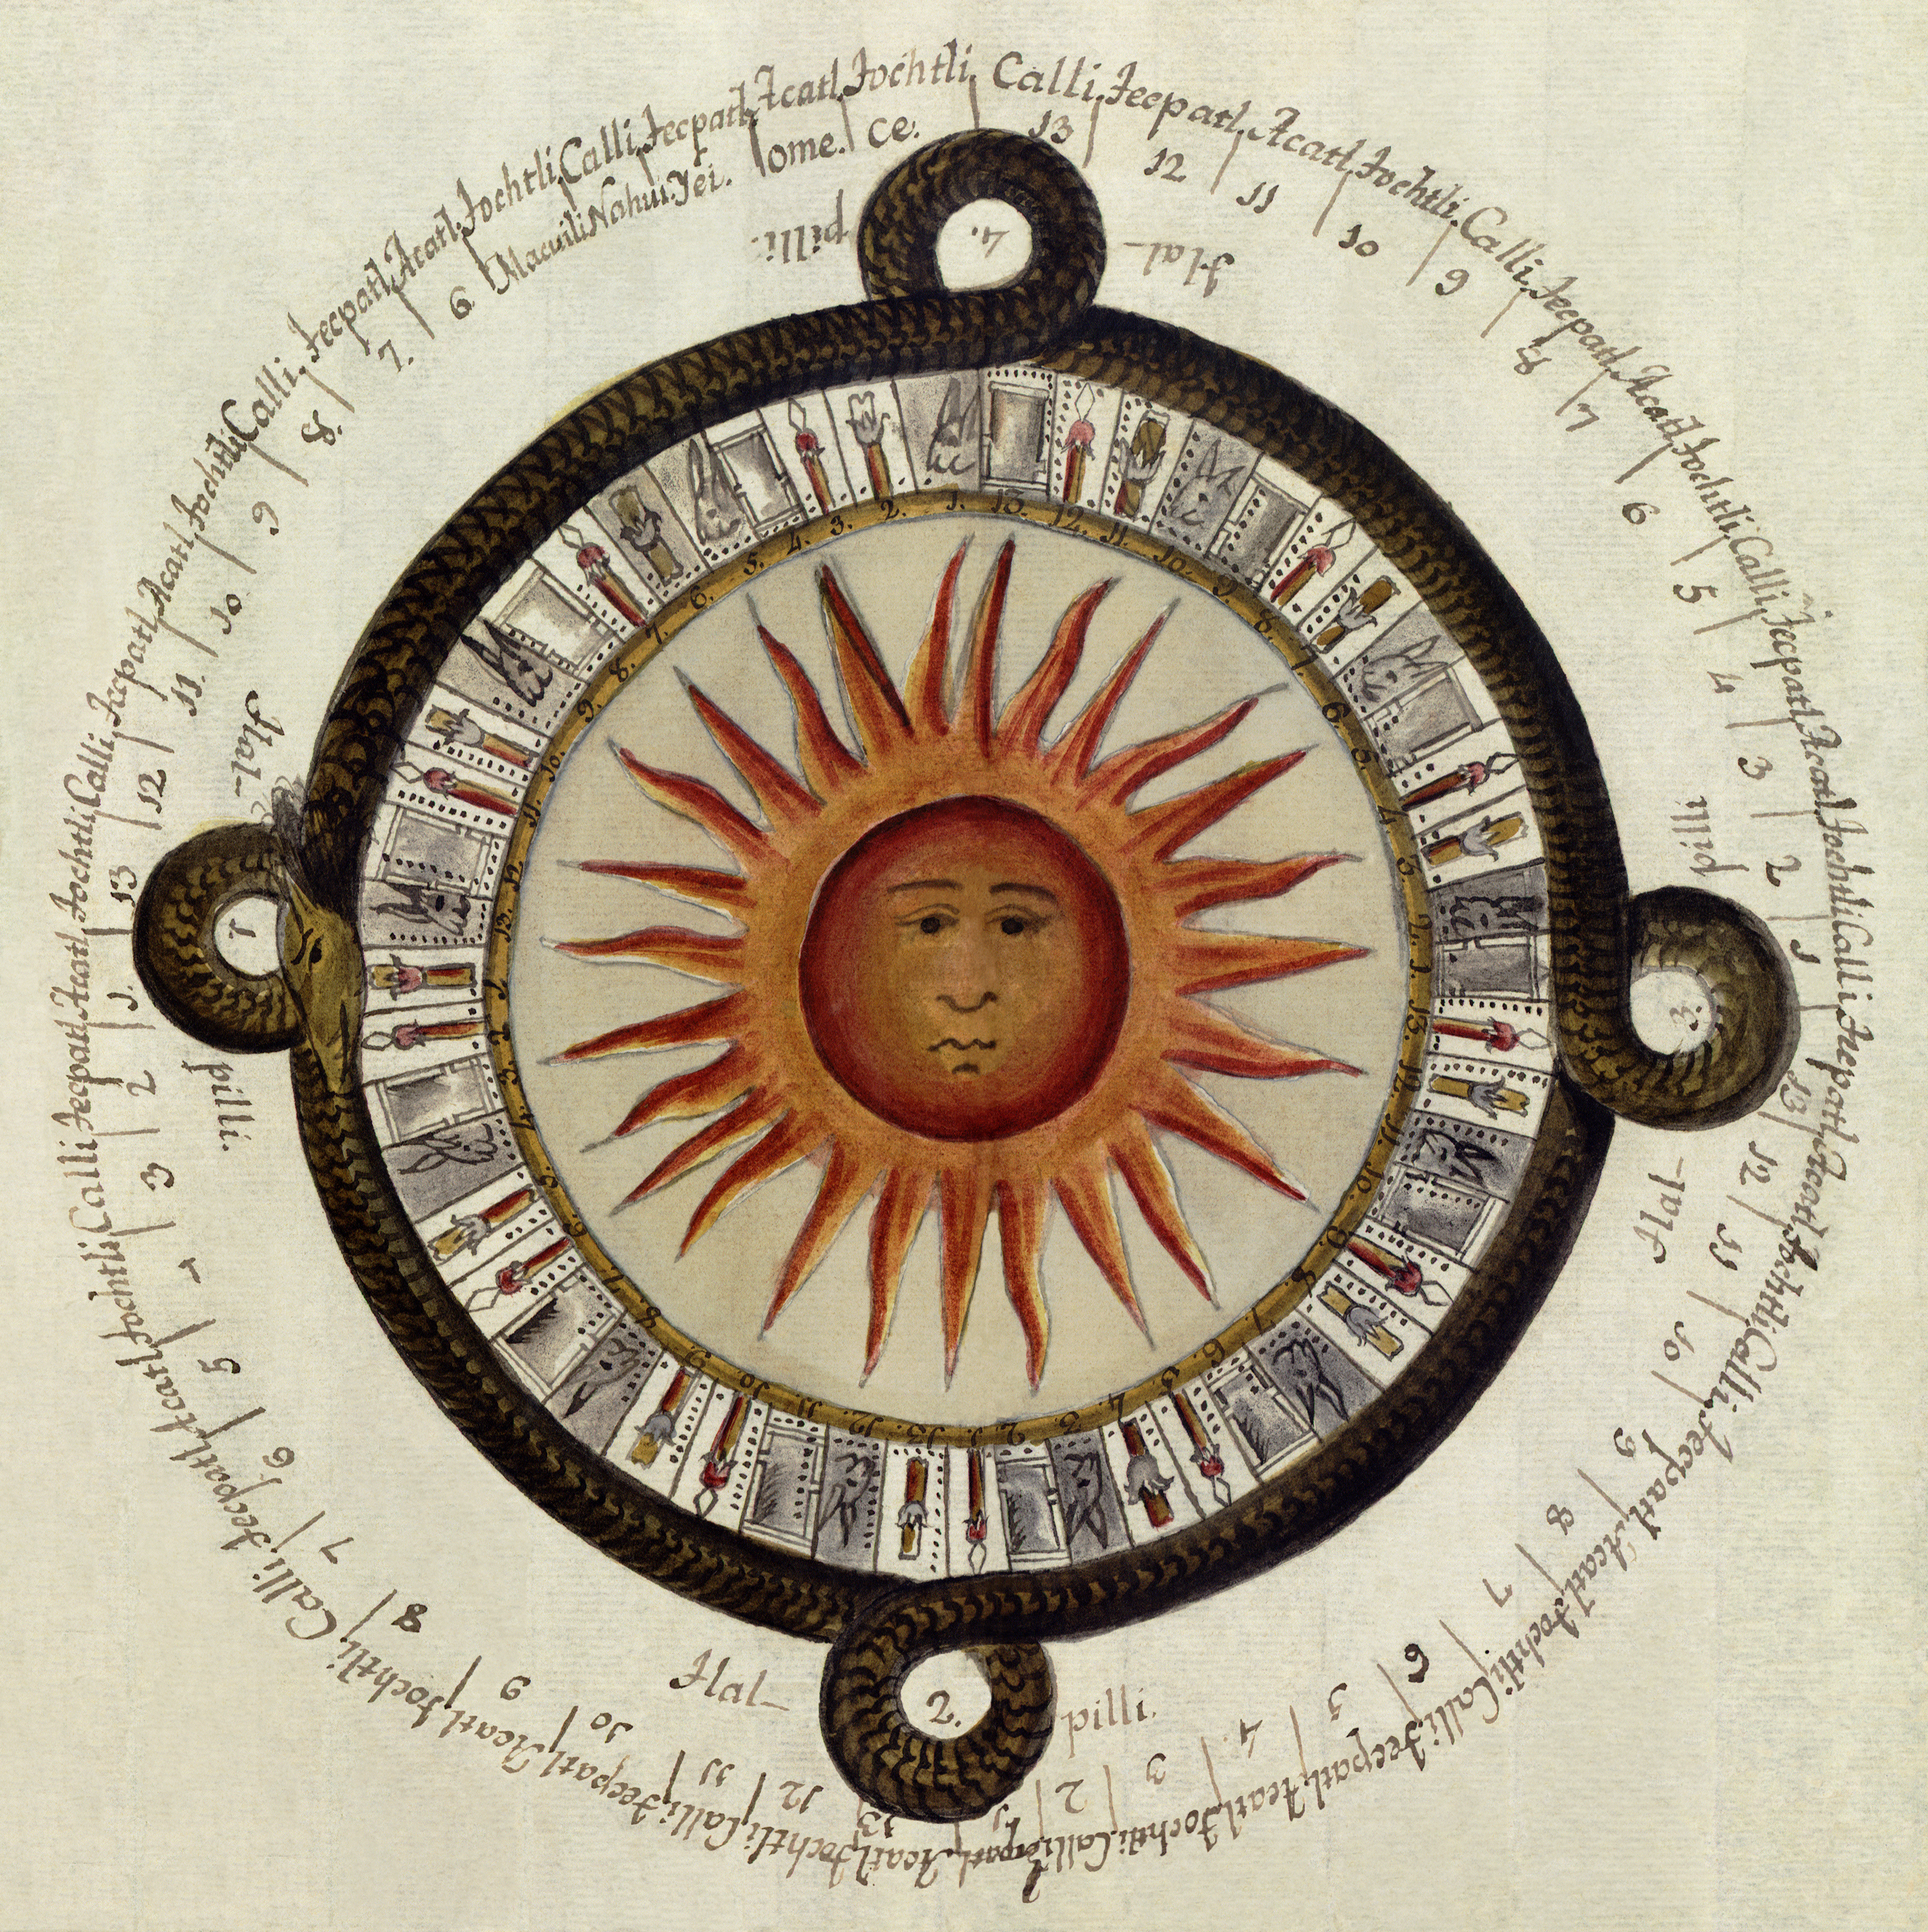
\includegraphics[width=2cm]{figures/sunstone.jpg}
\caption{\label{fig:leon} (Top) Leon}
\end{figure}
\begin{itemize}
\item La Coatlicue - An intact statue of the ``mother of the Gods,'' including Huitzilopochtli.
\item La Piedra del Sol - A calendar stone that led to a modern understanding of how the Aztec calendar worked.
\end{itemize}
\end{column}
\end{columns}
\end{frame}

\begin{frame}{More on Literary Societies and Journals}
\small
\begin{figure}
\includegraphics[width=0.4\textwidth]{figures/ab.jpg}
\caption{The colors of the aurora correspond to solar electrons interacting with various gases in the atmosphere.}
\end{figure}
\begin{enumerate}
\item European (French) scientists had established a lower limit on the latitude auroras could be observed: 35 degrees North of the Equator.
\item The Mexican scientists observed the aurora at 16.8 degrees North
\item Like modern scientists, they did not stop at observation but attempted to explain with a theoretical model
\end{enumerate}
\end{frame}

\begin{frame}{More on Literary Societies and Journals}
\small
\begin{figure}
\includegraphics[width=0.3\textwidth]{figures/earth-flare.jpg}
\includegraphics[width=0.4\textwidth]{figures/how-the-auroras-form.png}
\caption{(Left) The size of a coronal mass ejection is several times larger than Earth. (Right) The solar wind is charged, meaning it has a magnetic field, which adds to that of the Earth.}
\end{figure}
\begin{itemize}
\item Auroras are pretty, but they will kill you in your face
\item The three Mexican scientists noted that auroras were correlated with sun spots and provided historical data for future scientists
\item Increase in sun spot size, low altitude aurora
\end{itemize}
\end{frame}

\begin{frame}{More on Literary Societies and Journals}
\small
\begin{figure}
\includegraphics[width=0.4\textwidth]{figures/solar-max.jpg}
\includegraphics[width=0.33\textwidth]{figures/spot.jpg}
\caption{The colors of the aurora correspond to solar electrons interacting with various gases in the atmosphere.}
\end{figure}
\begin{itemize}
\item Sun spots are concentrations of magnetic field that deflect charged particle conduction
\item Cools the area, making it darker
\item Sun spots come in pairs (magnetic fields)
\end{itemize}
\end{frame}

\begin{frame}{More on Literary Societies and Journals}
\small
\begin{figure}
\includegraphics[width=0.3\textwidth]{figures/earth-flare.jpg}
\includegraphics[width=0.4\textwidth]{figures/how-the-auroras-form.png}
\caption{(Left) The size of a coronal mass ejection is several times larger than Earth. (Right) The solar wind is charged, meaning it has a magnetic field, which adds to that of the Earth.}
\end{figure}
\begin{itemize}
\item The scientists of New Spain deduced the altitude of the aurora phenomenon
\item Predicted where they could be observed in other continents, got some of them right
\end{itemize}
\end{frame}

\begin{frame}{More on Literary Societies and Journals}
\small
\begin{figure}
\includegraphics[width=0.3\textwidth]{figures/rad.jpg}
\includegraphics[width=0.4\textwidth]{figures/how-the-auroras-form.png}
\caption{(Left) The size of a coronal mass ejection is several times larger than Earth. (Right) The solar wind is charged, meaning it has a magnetic field, which adds to that of the Earth.}
\end{figure}
\begin{itemize}
\item They formulated a theory of how the light was produced, and designed an apparatus
\item Using the apparatus, \textbf{they reproduced some aurora properties in the lab.}
\end{itemize}
\end{frame}

\begin{frame}{More on Literary Societies and Journals}
\alert{Noteworthy for the history of science}: \\ \vspace{0.5cm}
\begin{quote}
De tres modelos originales de auroras boreales formulados en el continente americano hasta el siglo XVIII, dos de ellos fueron planteados en Nueva España y uno en Estados Unidos de Norteamérica [5].
\end{quote}
(Citing from paper above).  The results generated books, articles, and in particular, articles published in the journal founded by Alzate: \textit{Gacetas de Literatura.} \\
\textbf{Review graphs from paper.}
\end{frame}

\section{Colleges and Curricula}

\begin{frame}{Colleges and Curricula}

\end{frame}

\end{document}